\section{极限存在准则,两个重要极限}
\subsection{夹逼准则}
\begin{theorem}\label{theorem:极限.夹逼准则}
如果数列\(\{x_n\}\)、\(\{y_n\}\)及\(\{z_n\}\)满足下列条件:
\begin{enumerate}
	\item 从某项起,
	即\(\exists n_0 \in \mathbb{N}\),
	当\(n > n_0\)时,
	有\[
		y_n \leq x_n \leq z_n;
	\]

	\item \(\lim_{n\to\infty}{y_n}=a\),
	\(\lim_{n\to\infty}{z_n}=a\),
\end{enumerate}
那么数列\(\{x_n\}\)的极限存在,
且\(\lim_{n\to\infty}{x_n}=a\).
\begin{proof}
因为\(\lim_{n\to\infty}{y_n}=a\),
\(\lim_{n\to\infty}{z_n}=a\),
根据数列极限的定义,
有\[
	(\forall \epsilon > 0)
	(\exists N_1,N_2 \in \mathbb{N})
	(\forall n\in\mathbb{N})
	\left[
		\begin{array}{l}
			n > N_1 \implies \abs{y_n - a} < \epsilon, \\
			n > N_2 \implies \abs{z_n - a} < \epsilon
		\end{array}
	\right].
\]

现在取\(N = \max\{n_0,N_1,N_2\}\),
那么,当\(n > N\)时,有\[
	\left\{ \begin{array}{l}
		\abs{y_n - a} < \epsilon, \\
		\abs{z_n - a} < \epsilon,
	\end{array} \right.
	\quad\text{或}\quad
	\left\{ \begin{array}{l}
		a - \epsilon < y_n, \\
		z_n < a + \epsilon
	\end{array} \right.
\]同时成立.

又因当\(n > N\)时,有\[
	a - \epsilon < y_n \leq x_n \leq z_n < a + \epsilon,
\]即\[
	\abs{x_n - a} < \epsilon
\]成立.

综上所述,\[
	(\forall\epsilon>0)
	(\exists N\in\mathbb{N})
	(\forall n\in\mathbb{N})
	[
		n > N
		\implies
		\abs{x_n - a} < \epsilon
	];
\]
这就证明了\(\lim_{n\to\infty} x_n = a\).
\end{proof}
\end{theorem}

\begin{corollary}
如果
\begin{enumerate}
\item 当\(x \in \mathring{U}(x_0,\,r)\)(或\(\abs{x} > M\))时,\(g(x) \leq f(x) \leq h(x)\),
\item \(\lim_{x \to x_0} g(x) = A\)且\(\lim_{x \to x_0} h(x) = A\)(或\(\lim_{x \to \infty} g(x) = A\)且\(\lim_{x \to \infty} h(x) = A\)),
\end{enumerate}
那么\(\lim_{x \to x_0} f(x) = A\)(或\(\lim_{x \to \infty} f(x) = A\)).
\end{corollary}

\begin{example}
证明:\begin{equation}
	\lim_{n\to\infty} \sqrt[n]{k n} = 1
	\quad(k>0).
\end{equation}
\begin{proof}
当\(n \geq 3\)时,
将\(\sqrt[n]{k n}\)看作一个\(k\)、两个\(\sqrt{n}\)与\(n-3\)个\(1\)的几何平均值,
则有\[
	1 \leq \sqrt[n]{k n} = (k \cdot \sqrt{n}^2 \cdot 1^{n-3})^{1/n}
	< \frac{k + 2\sqrt{n} + n-3}{n}
	= 1 + \frac{2}{\sqrt{n}} + \frac{k-3}{n}.
\]
因为\[
	\lim_{n\to\infty} 1
	= \lim_{n\to\infty} \left(1 + \frac{2}{\sqrt{n}} + \frac{k-3}{n}\right) = 1,
\]
由夹逼定理可得\(\lim_{n\to\infty} \sqrt[n]{k n} = 1\).
\end{proof}
\end{example}

\begin{example}[重要极限I]
试证:\begin{equation}\label{equation:极限.重要极限I}
\lim_{x\to0} \frac{\sin x}{x} = 1.
\end{equation}
\begin{proof}
如图所示,
\begin{center}
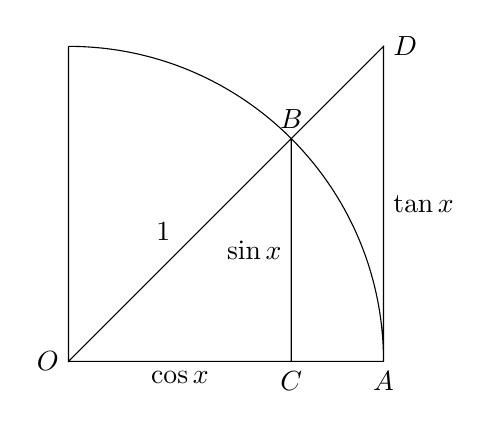
\begin{tikzpicture}
\pgfmathsetmacro{\r}{4}
\pgfmathsetmacro{\cx}{\r/sqrt(2)}
\coordinate (O) at (0,0);
\coordinate (A) at (\r,0);
\coordinate (B) at (\cx,\cx);
\coordinate (C) at (\cx,0);
\coordinate (D) at (\r,\r);
\draw (O)node[left]{\(O\)} -- (C)node[below]{\(C\)}node[midway,below]{\(\cos x\)} -- (A)node[below]{\(A\)}arc[start angle=0,end angle=90,radius=\r] (C) -- (B)node[above]{\(B\)}node[midway,left]{\(\sin x\)} -- (O)node[midway,above left]{\(1\)} -- (0,\r) (B) -- (D)node[right]{\(D\)} -- (A)node[midway,right]{\(\tan x\)};
\end{tikzpicture}
\end{center}
由于在\(0 < x < \pi/2\)时,\[
0 < \sin x < x < \tan x
\implies
1 < \frac{x}{\sin x} < \frac{1}{\cos x}
\implies
\cos x < \frac{\sin x}{x} < 1.
\]
因为\(\lim_{x\to0}\cos x = 1\),所以由\hyperref[theorem:极限.夹逼准则]{夹逼准则}可知,\(\lim_{x\to0} \frac{\sin x}{x} = 1\).
\end{proof}
\end{example}

\begin{figure}[ht]
	\centering
	\begin{tikzpicture}
		\begin{axis}[
			xmin=-4*pi,xmax=4*pi,
			ymin=-.5,ymax=1.2,
			width=\textwidth,
			height=.3\textheight,
			grid=both,
			xlabel=$x$,
			ylabel=$y$,
			enlargelimits,
			axis lines=middle,
			xtick={3.14,6.28,9.42,-3.14,-6.28,-9.42},
			xticklabels={$\pi$,$2\pi$,$3\pi$,$-\pi$,$-2\pi$,$-3\pi$},
		]
			\begin{scope}[samples=50,thick,red]
				\addplot[domain=.01:4*pi]{sin(deg(x))/x};
				\addplot[domain=-4*pi:-.01]{sin(deg(x))/x};
			\end{scope}
			\filldraw[draw=black,fill=white](0,1)circle(1pt);
		\end{axis}
	\end{tikzpicture}
	\caption{函数\(y=\frac{\sin x}{x}\)的图像}
	\label{figure:极限.函数[y=sin(x)/x]的图像}
\end{figure}

\begin{example}
\def\l{\lim_{x\to0}}
求:\(\l \frac{\tan x}{x}\).
\begin{solution}
\(
\l \frac{\tan x}{x}
= \l \left(\frac{\sin x}{x} \cdot \frac{1}{\cos x}\right)
= \l \frac{\sin x}{x} \cdot \lim_{x\to0}\frac{1}{\cos x}
= 1.
\)
\end{solution}
\end{example}

\begin{example}
\def\l{\lim_{x\to0}}
求:\(\l \frac{1 - \cos x}{x^2}\).
\begin{solution}
\(
\l \frac{1 - \cos x}{x^2}
= \l \frac{2 \sin^2\frac{x}{2}}{x^2}
= \frac{1}{2} \l \frac{\sin^2\frac{x}{2}}{\left(\frac{x}{2}\right)^2}
= \frac{1}{2} \left(\l \frac{\sin \frac{x}{2}}{\frac{x}{2}}\right)^2
= \frac{1}{2}.
\)
\end{solution}
\end{example}

\begin{example}
求:\(\lim_{x\to0}\frac{\arcsin x}{x}\).
\begin{solution}
令\(t = \arcsin x\),则\(x = \sin t\).当\(x\to0\)时,有\(t\to0\).于是由复合函数的极限运算法则得\[
\lim_{x\to0}\frac{\arcsin x}{x}
= \lim_{t\to0}\frac{t}{\sin t}
= 1.
\]
\end{solution}
\end{example}

\begin{example}
\def\l{\lim_{x\to0}}
计算\(\l \frac{\sin \omega x}{x}\).
\begin{solution}
当\(\omega=0\)时,\[
\l \frac{\sin \omega x}{x} = \l 0 = 0;
\]当\(\omega\neq0\)时,\[
\l \frac{\sin \omega x}{x}
= \omega \cdot \l \frac{\sin \omega x}{\omega x}
= \omega.
\]综上,\(\l \frac{\sin \omega x}{x} = \omega\).
\end{solution}
\end{example}

\begin{example}
\def\l{\lim_{x\to0}}
计算\(\l \frac{\sin mx}{\sin nx}\).
\begin{solution}
\(
\l \frac{\sin mx}{\sin nx}
= \frac{m}{n} \cdot \l \left( \frac{\sin mx}{mx} \cdot \frac{nx}{\sin nx} \right)
= \frac{m}{n}
\).
\end{solution}
\end{example}

\begin{example}
\def\l#1{\lim_{#1}}
计算\(\l{x\to\pi} \frac{\sin mx}{\sin nx} \quad(m,n\in\mathbb{Z})\).
\begin{solution}
\begin{align*}
\l{x\to\pi} \frac{\sin mx}{\sin nx}
&\xlongequal{t=x-\pi}
\l{t\to0} \frac{\sin m(t+\pi)}{\sin n(t+\pi)}
= \l{t\to0} \frac{(-1)^m}{(-1)^n} \frac{\sin mt}{\sin nt} \\
&= \l{t\to0} \frac{(-1)^m}{(-1)^n} \frac{\sin mt}{mt} \frac{m}{n} \frac{nt}{\sin nt}
= (-1)^{m-n} \frac{m}{n}.
\end{align*}
\end{solution}
\end{example}

\begin{example}
求:\(\lim_{n\to\infty}\frac{1 \cdot 3 \cdot 5 \dotsm (2n-1)}{2 \cdot 4 \cdot 6 \dotsm (2n)}\).
\begin{solution}
因为\((2n)^2 = 4n^2 > 4n^2-1 = (2n-1)(2n+1)\),\(2n > \sqrt{(2n-1)(2n+1)}\),所以\[
2 > \sqrt{1 \cdot 3},
4 > \sqrt{3 \cdot 5},
6 > \sqrt{5 \cdot 7},
\dotsc,
\]故\[
\frac{1 \cdot 3 \cdot 5 \dotsm (2n-1)}{2 \cdot 4 \cdot 6 \dotsm (2n)}
< \frac{1 \cdot 3 \cdot 5 \dotsm (2n-1)}{\sqrt{1 \cdot 3} \sqrt{3 \cdot 5} \sqrt{5 \cdot 7} \dotsm \sqrt{(2n-1)(2n+1)}}
= \frac{1}{\sqrt{2n+1}}.
\]

因为\(0 < \frac{1 \cdot 3 \cdot 5 \dotsm (2n-1)}{2 \cdot 4 \cdot 6 \dotsm (2n)} < \frac{1}{\sqrt{2n+1}}\),而\[
\lim_{n\to\infty}0 = \lim_{n\to\infty}\frac{1}{\sqrt{2n+1}} = 0,
\]所以\(\lim_{n\to\infty}\frac{1 \cdot 3 \cdot 5 \dotsm (2n-1)}{2 \cdot 4 \cdot 6 \dotsm (2n)} = 0\).
\end{solution}
\end{example}

\begin{example}
证明:\(\lim_{x\to0} \sqrt[n]{1+x} = 1\).
\begin{proof}
当\(x > 0\)时,
因为\(1 < \sqrt[n]{1+x} < 1+x\),
且\(\lim_{x\to0^+} 1 = \lim_{x\to0^+}(1+x) = 1\),
所以\[
	\lim_{x\to0^+} \sqrt[n]{1+x} = 1;
\]

当\(-1 < x < 0\)时,
因为\(1+x < \sqrt[n]{1+x} < 1\),
且\(\lim_{x\to0^-} 1 = \lim_{x\to0^-}(1+x) = 1\),
所以\[
	\lim_{x\to0^-} \sqrt[n]{1+x} = 1.
\]

综上,\(\lim_{x\to0} \sqrt[n]{1+x} = 1\).
\end{proof}
\end{example}

\begin{example}
证明:\(\lim_{x\to0^+} x \floor*{\frac{1}{x}} = 1\).
\begin{proof}
令\(t=1/x\),那么\[
x \floor*{\frac{1}{x}} = \frac{1}{t} \floor{t}.
\]又因为\[
t - 1 < \floor{t} \leq t,
\]\[
1 - \frac{1}{t} < \frac{1}{t} \floor{t} \leq 1;
\]而\[
\lim_{t\to+\infty} 1 - \frac{1}{t} = 1,
\quad
\lim_{t\to+\infty} 1 = 1,
\]所以\[
\lim_{x\to0^+} x \floor*{\frac{1}{x}} = \lim_{t\to+\infty} \frac{1}{t} \floor{t} = 1.
\qedhere
\]
\end{proof}
\end{example}

\begin{proposition}
设数列\(\{x_n\}\)满足\[
	\lim_{n\to\infty} \frac{x_{n+1}}{x_n} = \rho \in (-1,1),
\]
那么\(\lim_{n\to\infty} x_n = 0\).
\begin{proof}
因为\(\lim_{n\to\infty} \frac{x_{n+1}}{x_n} = \rho\),
所以根据数列极限的定义,
\(\forall\epsilon>0\),
\(\exists N\in\mathbb{N}\),
\(\forall n\in\mathbb{N}\),
只要\(n > N\),
就有\(\rho-\epsilon < \frac{x_{n+1}}{x_n} < \rho+\epsilon\).
取\(r=\max\{\abs{\rho-\epsilon},\abs{\rho+\epsilon}\}\),
那么有\(\abs{\frac{x_{n+1}}{x_n}} < r\),
即\(\abs{x_{n+1}} < r \abs{x_n}\),
于是\(0 \leq \abs{x_{n+k}} < r^k \abs{x_n}\ (k=1,2,\dotsc)\),
而\[
	\lim_{k\to\infty} r^k \abs{x_n} = 0,
\]
那么根据\hyperref[theorem:极限.夹逼准则]{夹逼准则},
\(\lim_{k\to\infty} \abs{x_{n+k}} = 0\),
因此\(\lim_{n\to\infty} x_n = 0\).
\end{proof}
\end{proposition}

\subsection{单调有界定理}
\begin{theorem}\label{theorem:极限.数列的单调有界定理}
单调有界数列必有极限.
\begin{proof}
不妨设数列\(\{a_n\}\)是单调增加的,即\[
	a_n \leq a_{n+1},
	\quad n=1,2,\dotsc;
	\eqno(1)
\]
又设\(\{a_n\}\)有界,且\[
	\abs{a_n} < c,
	\quad n=1,2,\dotsc.
	\eqno(2)
\]

现在我们把连续统分成两个集合\(A\)和\(B\),
把大于所有\(a_n\)的任何实数(例如数\(c\))放入集合\(B\),
而把其余的所有实数放入\(A\),即取\[
	B = \Set{ x \in \mathbb{R} \given x > a_n\ (n=1,2,\dotsc) },
	\eqno(3)
\]\[
	A = \mathbb{R} - B.
	\eqno(4)
\]
显然\(\Set{A,B}\)是\(\mathbb{R}\)的一个分割.
设\(\alpha\)是这个分割的界限,
那么必有\[
	a_n \leq \alpha,
	\quad n=1,2,\dotsc;
	\eqno(5)
\]
这是因为假设这个数列的某一项\(a_m\)满足\(a_m > \alpha\),
依照界限的定义会有\(a_m \in B\),而这与\(B\)的定义式(3)矛盾.

假设“\(\alpha\)不是\(\{a_n\}\)的极限”,
根据数列发散的定义,\[
	\exists\epsilon>0,
	\forall n\in\mathbb{N}^+,
	\exists n_0>n
	\bigl( \abs{a_{n_0} - \alpha} > \epsilon \bigr)
\]成立;
由(5)可知,\(\abs{a_{n_0} - \alpha} = \alpha - a_{n_0}\);
又因为\(\{a_n\}\)是单调增加的,
所以\(a_{n_0} \geq a_n\),
\(-a_{n_0} \leq -a_n\),
\(\alpha - a_{n_0} \leq \alpha - a_n\).
因此,\(\exists\epsilon>0\),对\(\forall n\in\mathbb{N}^+\),都有\[
	\alpha - a_n > \epsilon
	\quad\text{或}\quad
	a_n < \alpha - \epsilon.
	\eqno(6)
\]
结合集合\(B\)的定义(3),由(6)便得\(\alpha - \epsilon \in B\);
但由\(\alpha - \epsilon < \alpha\)可知,应该有\((\alpha - \epsilon) \in A\);
矛盾!因此假设不成立,\(\alpha\)就是数列\(\{a_n\}\)的极限,
即\(\lim_{n\to\infty} a_n = \alpha\).
\end{proof}
\end{theorem}

由\cref{theorem:极限.收敛数列的有界性} 可知,收敛的数列一定有界.
但是,我们也知道,有界的数列不一定收敛,例如\[
	\{ x_n = \sin n \}, \qquad
	\{ y_n = (-1)^n \}.
\]
现在\cref{theorem:极限.数列的单调有界定理} 表明:
如果数列不仅有界,而且是单调的,那么这数列的极限必定存在,也就是这数列一定收敛.

相应于单调有界数列必有极限的准则,函数极限也有类似的准则.
\begin{theorem}\label{theorem:极限.函数的单调有界定理}
设函数\(f(x)\)在点\(x_0\)的某个左邻域\((x_0-\delta,x_0)\)内单调并且有界,则\(f(x)\)在\(x_0\)的左极限\(f(x_0^-)\)必定存在.
\end{theorem}

\begin{example}[重要极限II]
试证:极限\(\lim_{x \to \infty}\left(1 + \frac{1}{x}\right)^x\)存在.
\begin{proof}
考虑\(x\)取正整数\(n\)而趋于\(+\infty\)的情形.设\(x_n=\left(1+\frac{1}{n}\right)^n\),根据牛顿二项公式,有\begin{align*}
x_n &= \left(1+\frac{1}{n}\right)^n
= \sum_{k=0}^n \frac{n!}{k! (n-k)!} \frac{1}{n^k} \\
&= 1 + \frac{n}{1!}\frac{1}{n} + \frac{n(n-1)}{2!}\frac{1}{n^2} + \frac{n(n-1)(n-2)}{3!}\frac{1}{n^3} + \dotsb \\
&\qquad+ \frac{n(n-1)\dotsm(n-n+1)}{n!}\frac{1}{n^n} \\
&= 1 + 1 + \frac{1}{2!}\left(1-\frac{1}{n}\right) + \frac{1}{3!}\left(1-\frac{1}{n}\right)\left(1-\frac{2}{n}\right) + \dotsb \\
&\qquad+ \frac{1}{n!}\left(1-\frac{1}{n}\right)\left(1-\frac{2}{n}\right)\dotsm\left(1-\frac{n-1}{n}\right),
\end{align*}
类似地,\begin{align*}
x_{n+1}
&= 1 + 1 + \frac{1}{2!}\left(1-\frac{1}{n+1}\right) + \frac{1}{3!}\left(1-\frac{1}{n+1}\right)\left(1-\frac{2}{n+1}\right) + \dotsb \\
&\qquad+ \frac{1}{n!}\left(1-\frac{1}{n+1}\right)\left(1-\frac{2}{n+1}\right)\dotsm\left(1-\frac{n-1}{n+1}\right) \\
&\qquad+ \frac{1}{(n+1)!}\left(1-\frac{1}{n+1}\right)\left(1-\frac{2}{n+1}\right)\dotsm\left(1-\frac{n}{n+1}\right),
\end{align*}
比较\(x_n\)和\(x_{n+1}\)的展开式,可以看到除前两项外,\(x_n\)的每一项都小于\(x_{n+1}\)的对应项,并且\(x_{n+1}\)还多了最后一项\[
\frac{1}{(n+1)!}\left(1-\frac{1}{n+1}\right)\left(1-\frac{2}{n+1}\right)\dotsm\left(1-\frac{n}{n+1}\right) > 0,
\]因此\[
x_n < x_{n+1},
\]这就说明数列\(\{x_n\}\)是单调增加的.

又因为\[
x_n < 1 + 1 + \frac{1}{2!} + \frac{1}{3!} + \dotsb + \frac{1}{n!}
< 1 + 1 + \frac{1}{2} + \frac{1}{2^2} + \dotsb + \frac{1}{2^{n-1}}
= 3 - \frac{1}{2^{n-1}} < 3,
\]这就说明数列\(\{x_n\}\)是有界的.

既然数列\(\{x_n\}\)是单调增加的,
又是有界的,
那么数列\(\{x_n\}\)的极限一定存在,
记它的极限值为常数\(e\).

再设\(n \leq x < n+1\),则\[
\left(1+\frac{1}{n+1}\right)^n < \left(1+\frac{1}{x}\right)^x < \left(1+\frac{1}{n}\right)^{n+1},
\]且当\(n\to\infty\)时,\(x\to\infty\),而\[
\lim_{n\to\infty}\left(1+\frac{1}{n+1}\right)^n
=\lim_{n\to\infty}\frac{\left(1+\frac{1}{n+1}\right)^{n+1}}{1+\frac{1}{n+1}} = e,
\]\[
\lim_{n\to\infty}\left(1+\frac{1}{n}\right)^{n+1}
=\lim_{n\to\infty}\left[\left(1+\frac{1}{n}\right)^n\cdot\left(1+\frac{1}{n}\right)\right]=e,
\]应用\hyperref[theorem:极限.夹逼准则]{夹逼准则}可得\[
\lim_{x\to+\infty}\left(1+\frac{1}{x}\right)^x = e.
\]令\(x=-(t+1)\),则\(x\to-\infty\)时,\(t\to+\infty\),从而\begin{align*}
\lim_{x\to-\infty}\left(1+\frac{1}{x}\right)^x
&=\lim_{t\to+\infty}\left(1-\frac{1}{t+1}\right)^{-(t+1)}
=\lim_{t\to+\infty}\left(\frac{t}{t+1}\right)^{-(t+1)} \\
&=\lim_{t\to+\infty}\left(1+\frac{1}{t}\right)^{t+1}
=\lim_{t\to+\infty}\left[\left(1+\frac{1}{t}\right)^t\cdot\left(1+\frac{1}{t}\right)\right]=e.
\end{align*}

综上所述,由于\[
\lim_{x\to+\infty}\left(1+\frac{1}{x}\right)^x
= \lim_{x\to-\infty}\left(1+\frac{1}{x}\right)^x
= e,
\]所以\begin{equation}\label{equation:极限.重要极限II}
\lim_{x\to\infty} \left(1+\frac{1}{x}\right)^x = e.
\end{equation}
这就说明函数极限\(\lim_{x\to\infty} \left(1+\frac{1}{x}\right)^x\)存在.
\end{proof}
\end{example}
我们称上面所说的常数\(e\)为“\DefineConcept{欧拉常数} \(e\)”.

另外,利用复合函数的极限运算法则,可得
\begin{equation}
\lim_{z\to0}(1+z)^{\frac{1}{z}}
\xlongequal{z=1/x}
\lim_{x\to\infty}\left(1+\frac{1}{x}\right)^x
= e.
\end{equation}

\begin{figure}[ht]
	\centering
	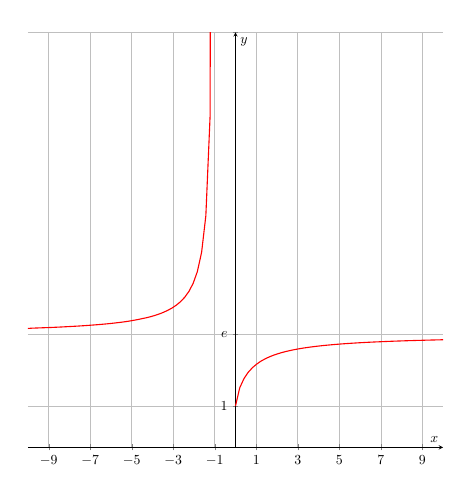
\begin{tikzpicture}[scale=.5]
	% Mathematica: Plot[{E,(1+1/x)^x},{x,-10,10},PlotRange->{0,10},AspectRatio->Automatic,PlotStyle->{{Dashed,Thin},Thin}]
		\begin{axis}[
			xmin=-10,xmax=10,ymin=0,ymax=10,
			grid=both,width=\textwidth,height=\textwidth,
			xlabel=$x$,
			ylabel=$y$,
			enlarge x limits=0.1,
			enlarge y limits=0.1,
			axis lines = middle,
			xtick={-9,-7,...,9},
			ytick={1,2.718,10},
			yticklabels={$1$,$e$},
		]
			\begin{scope}[samples=50,thick,red]
				\addplot[domain=-10:-0]{(1+1/x)^x};
				\addplot[domain=+0:+10]{(1+1/x)^x};
			\end{scope}
		\end{axis}
	\end{tikzpicture}
	\caption{函数\(y=\left(1+\tfrac{1}{x}\right)^x\)的图像}
	\label{figure:极限.函数(1+1/x)^x的图像}
\end{figure}

如\cref{figure:极限.函数(1+1/x)^x的图像} 所示,
我们可以画出函数\(y=\left(1+\frac{1}{x}\right)^x\ (x<-1 \lor x>0)\)的图像.
可见,直线\(y=e\)是函数\(y=\left(1+\frac{1}{x}\right)^x\)的图像的水平渐近线.
另外,易证\[
\lim_{x\to0^+} \left(1+\frac{1}{x}\right)^x = 1,
\qquad
\lim_{x\to1^-} \left(1+\frac{1}{x}\right)^x = +\infty.
\]


\begin{example}
求:\(\lim_{x \to \infty}\left(1 - \frac{1}{x}\right)^x\).
\begin{solution}
令\(t = -x\),则当\(x \to +\infty\)时,\(t \to -\infty\),于是\[
\lim_{x \to +\infty}\left(1 - \frac{1}{x}\right)^x
= \lim_{t \to -\infty}\left(1 + \frac{1}{t}\right)^{-t}
= \lim_{t \to -\infty}\frac{1}{\left(1 + \frac{1}{t}\right)^t}
= \frac{1}{e}.
\]
\end{solution}

画出函数\(y=\left(1-\frac{1}{x}\right)^x\ (x<0 \lor x\geq1)\)的图像如\cref{figure:极限.函数(1-1/x)^x的图像}.
\begin{figure}[ht]
	\centering
	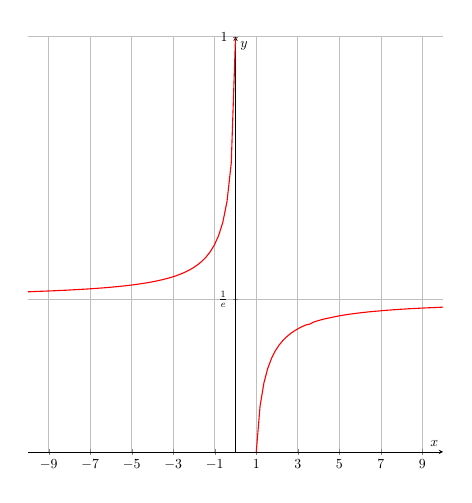
\begin{tikzpicture}[scale=.5]
		% Mathematica: Plot[{1/E, (1 - 1/x)^x}, {x, -10, 10}, PlotRange -> {0, 1}, PlotStyle -> {{Dashed, Thin}, Thin}]
		\begin{axis}[
			xmin=-10,xmax=10,
			ymin=0,ymax=1,
			grid=both,
			width=\textwidth,height=\textwidth,
			xlabel=$x$,
			ylabel=$y$,
			axis lines=middle,
			xtick={-9,-7,...,10},
			ytick={.3679,1},
			yticklabels={$\frac{1}{e}$,$1$},
		]
			\begin{scope}[samples=50,thick,red]
				\addplot[domain=-10:-0]{(1-1/x)^x};
				\addplot[domain=+1:+10]{(1-1/x)^x};
			\end{scope}
		\end{axis}
	\end{tikzpicture}
	\caption{函数\(y=\left(1-\tfrac{1}{x}\right)^x\)的图像}
	\label{figure:极限.函数(1-1/x)^x的图像}
\end{figure}
可见,直线\(y=\frac{1}{e}\)是函数\(y=\left(1-\frac{1}{x}\right)^x\)的图像的水平渐近线.
另外,易证\[
	\lim_{x\to0^-} \left(1-\frac{1}{x}\right)^x
	\xlongequal{t=-1/x} \lim_{t\to+\infty} \frac{1}{\sqrt[t]{1+t}}
	= 1.
\]
\end{example}

\subsection{柯西极限存在准则}

\begin{theorem}[柯西极限存在准则]\label{theorem:极限.数列的柯西极限存在准则}
%@see: 《高等数学(第六版 上册)》 P55 柯西极限存在准则
数列\(\{x_n\}\)收敛的充分必要条件是:
对于任意给定的正数\(\epsilon\),
存在正整数\(N\),
使得当\(m>N\)且\(n>N\)时,
就有\(\abs{x_n-x_m}<\epsilon\).
\begin{proof}
必要性.
设\(\lim_{n\to\infty}x_n = a\).
由数列极限的定义,
对于\(\forall\epsilon>0\),
\(\exists N \in \mathbb{N}^+\),
当\(n > N\)时,有\[
	\abs{x_n - a} < \frac{\epsilon}{2};
\]
同样地,当\(m > N\)时,有\[
	\abs{x_m - a} < \frac{\epsilon}{2}.
\]
因此,当\(n > N\)且\(m > N\)时,有\[
	\abs{x_n - x_m} = \abs{(x_n - a) - (x_m - a)}
	\leq \abs{x_n - a} + \abs{x_m - a}
	< \frac{\epsilon}{2} + \frac{\epsilon}{2}
	= \epsilon.
	\qedhere
\]
%TODO 未证充分性
\end{proof}
\end{theorem}
柯西极限存在准则有时也叫作\DefineConcept{柯西审敛原理}.

它可以用“\(\epsilon-\delta\)”语言表示为:\[
	\text{数列\(\{x_n\}\)收敛}
	\iff
	(\forall\epsilon>0)
	(\exists N\in\mathbb{N})
	(\forall n,m \geq N)
	[\abs{x_n-x_m}<\epsilon].
\]

类似地,函数极限也有自己的柯西审敛原理.

\begin{definition}\label{definition:极限.函数在集合上的振幅}
%@see: 《数学分析》(卓里奇) P109 定义16.
对于任意一个函数\(f\colon X\to\mathbb{R}\),
集合\(E \subseteq X\),
定义:\[
	\amp(f;E)
	\defeq
	\sup_{x_1,x_2 \in E}\abs{f(x_1)-f(x_2)},
\]
称为“函数\(f\)在集合\(E\)上的\DefineConcept{振幅}”.
\end{definition}

\begin{theorem}\label{theorem:极限.函数的柯西极限存在准则}
函数\(f(x)\)在点\(a\)的极限存在的充分必要条件是:
对于任意给定的正数\(\epsilon\),
存在正数\(\delta\),
使得当\(0 < \abs{x_1 - a} < \delta\)且\(0 < \abs{x_2 - a} < \delta\)时,
就有\(\abs{f(x_1) - f(x_2)} < \epsilon\).
\end{theorem}

